\section{Results}
\label{results}
In this section I will discuss the balancing results for the two main algorithms I tested the pass on: RC4 and AES.
Both algorithms have been written/adapted so that they utilize the stack as much as possible, maximizing the benefit of my balancing pass.

\subsection{Security}
\begin{figure}[h]
  \centering
  \begin{subfigure}[b]{0.49\textwidth}
    % This file was created by matplotlib2tikz v0.7.4.
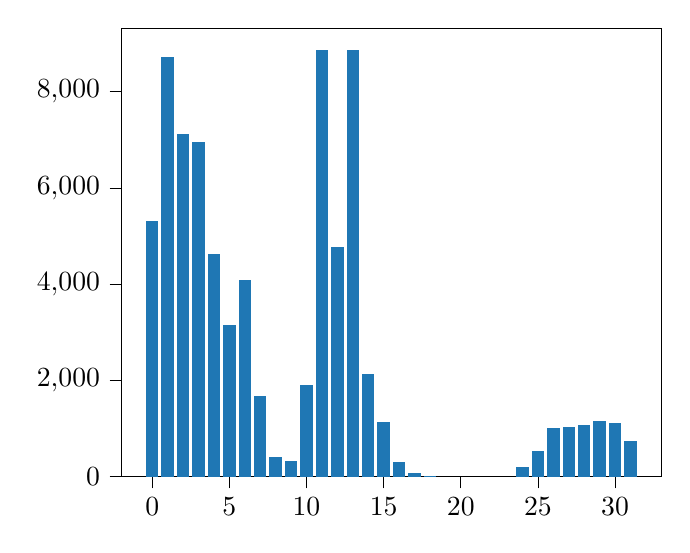
\begin{tikzpicture}

\definecolor{color0}{rgb}{0.12156862745098,0.466666666666667,0.705882352941177}

\begin{axis}[
tick align=outside,
tick pos=left,
x grid style={white!69.01960784313725!black},
xmin=-1.99, xmax=32.99,
xtick style={color=black},
y grid style={white!69.01960784313725!black},
ymin=0, ymax=9319.8,
ytick style={color=black}
]
\draw[fill=color0,draw opacity=0] (axis cs:-0.4,0) rectangle (axis cs:0.4,5313);
\draw[fill=color0,draw opacity=0] (axis cs:0.6,0) rectangle (axis cs:1.4,8720);
\draw[fill=color0,draw opacity=0] (axis cs:1.6,0) rectangle (axis cs:2.4,7129);
\draw[fill=color0,draw opacity=0] (axis cs:2.6,0) rectangle (axis cs:3.4,6958);
\draw[fill=color0,draw opacity=0] (axis cs:3.6,0) rectangle (axis cs:4.4,4620);
\draw[fill=color0,draw opacity=0] (axis cs:4.6,0) rectangle (axis cs:5.4,3153);
\draw[fill=color0,draw opacity=0] (axis cs:5.6,0) rectangle (axis cs:6.4,4082);
\draw[fill=color0,draw opacity=0] (axis cs:6.6,0) rectangle (axis cs:7.4,1682);
\draw[fill=color0,draw opacity=0] (axis cs:7.6,0) rectangle (axis cs:8.4,413);
\draw[fill=color0,draw opacity=0] (axis cs:8.6,0) rectangle (axis cs:9.4,319);
\draw[fill=color0,draw opacity=0] (axis cs:9.6,0) rectangle (axis cs:10.4,1911);
\draw[fill=color0,draw opacity=0] (axis cs:10.6,0) rectangle (axis cs:11.4,8873);
\draw[fill=color0,draw opacity=0] (axis cs:11.6,0) rectangle (axis cs:12.4,4778);
\draw[fill=color0,draw opacity=0] (axis cs:12.6,0) rectangle (axis cs:13.4,8876);
\draw[fill=color0,draw opacity=0] (axis cs:13.6,0) rectangle (axis cs:14.4,2142);
\draw[fill=color0,draw opacity=0] (axis cs:14.6,0) rectangle (axis cs:15.4,1133);
\draw[fill=color0,draw opacity=0] (axis cs:15.6,0) rectangle (axis cs:16.4,312);
\draw[fill=color0,draw opacity=0] (axis cs:16.6,0) rectangle (axis cs:17.4,82);
\draw[fill=color0,draw opacity=0] (axis cs:17.6,0) rectangle (axis cs:18.4,9);
\draw[fill=color0,draw opacity=0] (axis cs:18.6,0) rectangle (axis cs:19.4,0);
\draw[fill=color0,draw opacity=0] (axis cs:19.6,0) rectangle (axis cs:20.4,0);
\draw[fill=color0,draw opacity=0] (axis cs:20.6,0) rectangle (axis cs:21.4,0);
\draw[fill=color0,draw opacity=0] (axis cs:21.6,0) rectangle (axis cs:22.4,0);
\draw[fill=color0,draw opacity=0] (axis cs:22.6,0) rectangle (axis cs:23.4,0);
\draw[fill=color0,draw opacity=0] (axis cs:23.6,0) rectangle (axis cs:24.4,208);
\draw[fill=color0,draw opacity=0] (axis cs:24.6,0) rectangle (axis cs:25.4,524);
\draw[fill=color0,draw opacity=0] (axis cs:25.6,0) rectangle (axis cs:26.4,1004);
\draw[fill=color0,draw opacity=0] (axis cs:26.6,0) rectangle (axis cs:27.4,1023);
\draw[fill=color0,draw opacity=0] (axis cs:27.6,0) rectangle (axis cs:28.4,1064);
\draw[fill=color0,draw opacity=0] (axis cs:28.6,0) rectangle (axis cs:29.4,1157);
\draw[fill=color0,draw opacity=0] (axis cs:29.6,0) rectangle (axis cs:30.4,1123);
\draw[fill=color0,draw opacity=0] (axis cs:30.6,0) rectangle (axis cs:31.4,741);
\end{axis}

\end{tikzpicture}
    \caption{Unbalanced RC4}
  \end{subfigure}
  \begin{subfigure}[b]{0.49\textwidth}
    % This file was created by matplotlib2tikz v0.7.4.
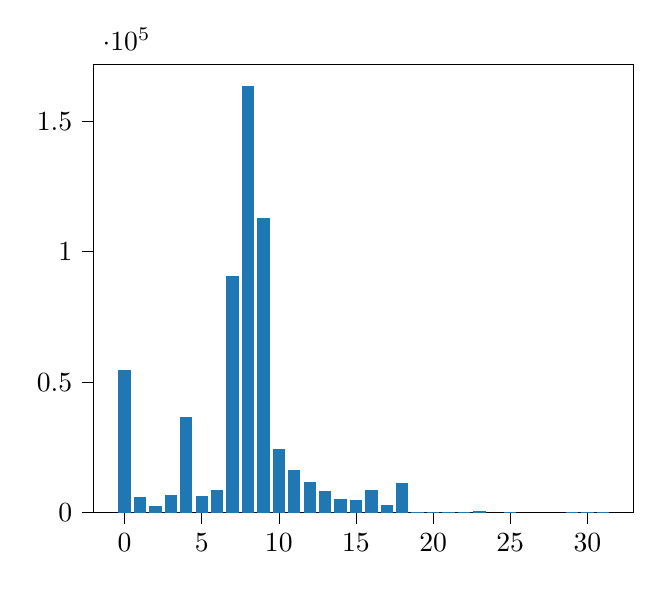
\begin{tikzpicture}

\definecolor{color0}{rgb}{0.12156862745098,0.466666666666667,0.705882352941177}

\begin{axis}[
tick align=outside,
tick pos=left,
x grid style={white!69.01960784313725!black},
xmin=-1.99, xmax=32.99,
xtick style={color=black},
y grid style={white!69.01960784313725!black},
ymin=0, ymax=171938.55,
ytick style={color=black}
]
\draw[fill=color0,draw opacity=0] (axis cs:-0.4,0) rectangle (axis cs:0.4,54571);
\draw[fill=color0,draw opacity=0] (axis cs:0.6,0) rectangle (axis cs:1.4,6050);
\draw[fill=color0,draw opacity=0] (axis cs:1.6,0) rectangle (axis cs:2.4,2313);
\draw[fill=color0,draw opacity=0] (axis cs:2.6,0) rectangle (axis cs:3.4,6824);
\draw[fill=color0,draw opacity=0] (axis cs:3.6,0) rectangle (axis cs:4.4,36773);
\draw[fill=color0,draw opacity=0] (axis cs:4.6,0) rectangle (axis cs:5.4,6353);
\draw[fill=color0,draw opacity=0] (axis cs:5.6,0) rectangle (axis cs:6.4,8761);
\draw[fill=color0,draw opacity=0] (axis cs:6.6,0) rectangle (axis cs:7.4,90865);
\draw[fill=color0,draw opacity=0] (axis cs:7.6,0) rectangle (axis cs:8.4,163751);
\draw[fill=color0,draw opacity=0] (axis cs:8.6,0) rectangle (axis cs:9.4,112999);
\draw[fill=color0,draw opacity=0] (axis cs:9.6,0) rectangle (axis cs:10.4,24463);
\draw[fill=color0,draw opacity=0] (axis cs:10.6,0) rectangle (axis cs:11.4,16480);
\draw[fill=color0,draw opacity=0] (axis cs:11.6,0) rectangle (axis cs:12.4,11631);
\draw[fill=color0,draw opacity=0] (axis cs:12.6,0) rectangle (axis cs:13.4,8125);
\draw[fill=color0,draw opacity=0] (axis cs:13.6,0) rectangle (axis cs:14.4,5158);
\draw[fill=color0,draw opacity=0] (axis cs:14.6,0) rectangle (axis cs:15.4,4929);
\draw[fill=color0,draw opacity=0] (axis cs:15.6,0) rectangle (axis cs:16.4,8458);
\draw[fill=color0,draw opacity=0] (axis cs:16.6,0) rectangle (axis cs:17.4,2812);
\draw[fill=color0,draw opacity=0] (axis cs:17.6,0) rectangle (axis cs:18.4,11488);
\draw[fill=color0,draw opacity=0] (axis cs:18.6,0) rectangle (axis cs:19.4,374);
\draw[fill=color0,draw opacity=0] (axis cs:19.6,0) rectangle (axis cs:20.4,342);
\draw[fill=color0,draw opacity=0] (axis cs:20.6,0) rectangle (axis cs:21.4,206);
\draw[fill=color0,draw opacity=0] (axis cs:21.6,0) rectangle (axis cs:22.4,170);
\draw[fill=color0,draw opacity=0] (axis cs:22.6,0) rectangle (axis cs:23.4,456);
\draw[fill=color0,draw opacity=0] (axis cs:23.6,0) rectangle (axis cs:24.4,0);
\draw[fill=color0,draw opacity=0] (axis cs:24.6,0) rectangle (axis cs:25.4,179);
\draw[fill=color0,draw opacity=0] (axis cs:25.6,0) rectangle (axis cs:26.4,0);
\draw[fill=color0,draw opacity=0] (axis cs:26.6,0) rectangle (axis cs:27.4,0);
\draw[fill=color0,draw opacity=0] (axis cs:27.6,0) rectangle (axis cs:28.4,2);
\draw[fill=color0,draw opacity=0] (axis cs:28.6,0) rectangle (axis cs:29.4,8);
\draw[fill=color0,draw opacity=0] (axis cs:29.6,0) rectangle (axis cs:30.4,41);
\draw[fill=color0,draw opacity=0] (axis cs:30.6,0) rectangle (axis cs:31.4,16);
\end{axis}

\end{tikzpicture}

    \caption{Balanced RC4}
  \end{subfigure}

  \begin{subfigure}[b]{\textwidth}
    \begin{tikzpicture}
\begin{axis}[
    ybar=2*\pgflinewidth,
    bar width=0.00725\textwidth,
    enlargelimits=0.05,
    xtick={0,8,16,24,32},
    width=\textwidth,
    xlabel={\hammingw{}},
    ylabel={Fraction of Occurences},
]
\addplot[pantone289,fill=pantone289!40] table [x=i, y=unbalanced-scaled, col sep=comma] {data/rc4.csv};
\addplot[pantone144,fill=pantone144!40] table [x=i, y=balanced-scaled, col sep=comma] {data/rc4.csv};
\legend{Unbalanced,Balanced}
\end{axis}
\end{tikzpicture}

    \caption{Scaled Hamming weight histograms for RC4}
  \end{subfigure}
  \caption{Hamming weight histograms for balanced and unbalanced RC4}
\end{figure}

\begin{figure}[h]
  \centering
  \begin{subfigure}[b]{0.49\textwidth}
    \input{tikz/aes-unbalanced.tex}
    \caption{Unbalanced AES}
  \end{subfigure}
  \begin{subfigure}[b]{0.49\textwidth}
    \begin{tikzpicture}
\begin{axis}[
    ybar,
    bar width=0.015\textwidth,
    enlargelimits=0.05,
    xtick={0,8,16,24,32},
    width=\textwidth,
    xlabel={\hammingw{}},
    ylabel={Occurences}
]
\addplot[pantone289,fill=pantone289!40] table [x=i, y=balanced-total, col sep=comma] {data/aes.csv};
\end{axis}
\end{tikzpicture}

    \caption{Balanced AES}
  \end{subfigure}

  \begin{subfigure}[b]{\textwidth}
    \input{tikz/aes-comparison.tex}
    \caption{Scaled Hamming weight histograms for AES}
  \end{subfigure}
  \caption{Hamming weight histograms for balanced and unbalanced AES}
\end{figure}

\subsection{Performance}
aoeu
